\documentclass[../thesis.tex]{subfiles}

\begin{document}

\chapter{Reactor antineutrino prediction}
\label{chap:reactor}

\begin{comment}
Note to self: See Kam-Biu's comments on first page of Reactor.pdf. Add SNF plot from DocDB. Also NE corrections (tabulate or plot, take from [Lewis] or [Mueller]?)
\end{comment}

In principle, a reactor-based near/far experiment can measure the oscillation parameters without any recourse to reactor physics: Simply measure the spectrum of the $\nuebar$s at the near site, ``unoscillate'' it back to the reactor, and then oscillate it out to the far site. The oscillation parameters are then those that give the best fit to the far-site data. No information is needed on the reactor power, fission fractions, or theoretical antineutrino spectra.

In practice, the situation is complicated by the fact that Daya Bay features three reactor complexes and two near sites. Instead of two baselines, there are effectively nine, and the reactors can differ from each other in terms of instantaneous power and burnup. These factors must be accounted for when predicting the far-site $\nuebar$ spectra from the near ones.

In the simplest approach, one can just use the known operating power and baseline information to split each near $\nuebar$ spectrum into components from each reactor, and then unoscillate/oscillate each component separately to the far site. This can be done separately for each near site, and the two far-site predictions can then be averaged. This is sufficient for getting a good measurement of $\theta_{13}$, thanks to the cancellation of absolute efficiency uncertainties and the lack of need for reactor modeling.

However, measuring $\Delta m^2$ involves examining the detailed shapes of the near and far spectra. In the simple approach just described, it is assumed that all reactors are producing the same spectral shape (and ratio of $\nuebar$ flux to reactor power). This is not necessarily accurate, as the reactors may be in different stages of their fuel cycles. Therefore, to get the most out of a rate/shape analysis, we must perform a full prediction of the spectrum from each reactor separately. This will, naturally, introduce uncertainties from the imperfect nature of the predictions. As long as the predictions are applied consistently, their uncertainties will be largely (but not completely) cancelled in the near/far ratios, so this primary benefit of a near/far measurement is not lost.

This chapter describes the reactor prediction, beginning with the question of predicting the antineutrino spectrum from a single fission of a given isotope, and then proceeding to discuss how these are combined, with the aid of information on generated thermal power and burnup (i.e., fission fractions), to form a full spectrum prediction.

\section{Spectrum prediction}
\label{sec:specpred}

\def\urfive{$^{235}$U\xspace} \def\punine{$^{239}$Pu\xspace}
\def\puone{$^{241}$Pu\xspace} \def\ureight{$^{238}$U\xspace}

In a conventional pressurized water reactor, each megawatt of thermal power corresponds to about $2\times10^{20}$ fissions per second, with each fission producing an average of about six antineutrinos from the beta decays of the fission fragments (or their daughters) \cite{PhysRevC.84.024617}. Virtually all of the power originates from the fission of four isotopes: \urfive, \punine, \puone, and \ureight. In a fresh fuel assembly of low-enriched (3--5\% $^{235}$U) uranium, initially some 92\% of fissions will be of \urfive, while the remaining 8\% will be fast-neutron fissions of \ureight. This \ureight fraction remains nearly constant throughout a fuel cycle. At the same time, some of the \ureight will undergo neutron capture and subsequent beta decay to \punine, whose fission rate rapidly reaches 10-20\% of the total, eventually catching up to the (decreasing) \urfive rate by the end of the cycle ($\sim$450 days). A fraction of \punine will produce \puone after a pair of neutron captures, and by the end of the cycle this isotope will contribute a fission fraction comparable to that of \ureight. This evolution of the fission fractions is illustrated in \autoref{fig:reacFissionFrac}.

\begin{figure}[ht]
  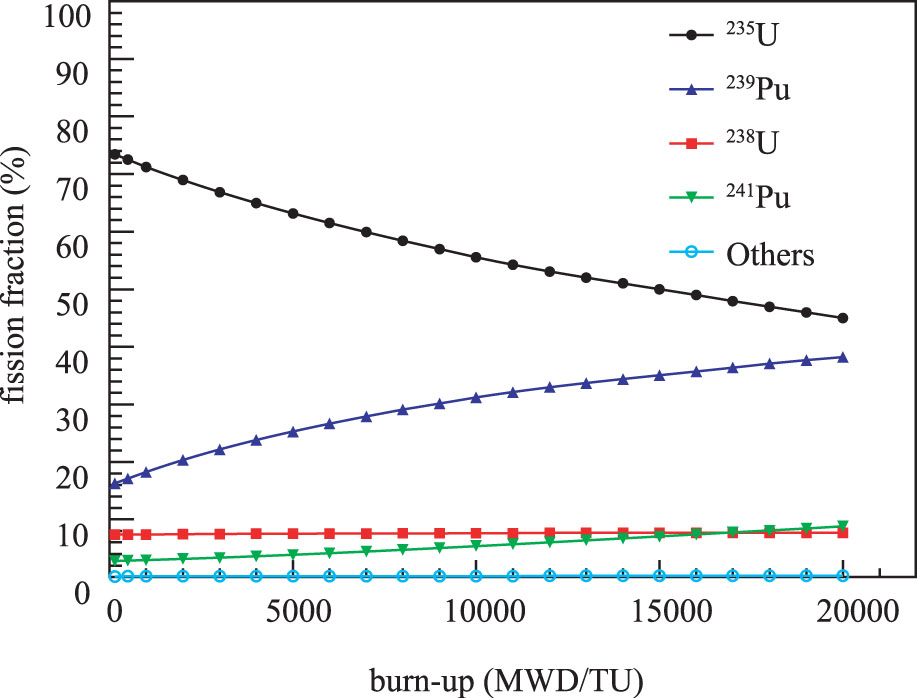
\includegraphics[width=0.6\textwidth]{Reactor/fission_frac.jpg}
  \caption{Fission fractions over time in a typical pressurized water reactor. From \cite{spectrum2017}.}
  \label{fig:reacFissionFrac}
\end{figure}

Clearly, all four isotopes contribute a non-neglible fraction of the total thermal power, and since their antineutrino spectra are fairly similar, they all contribute significantly to the flux. Therefore, it is imperative that each isotope's spectrum be predicted accurately. This can be done either \emph{ab initio}, by summing theoretical spectra based on the individual beta-decay branches of all fission products listed in nuclear databases, or via the \emph{conversion method}, in which the total beta-ray spectrum is measured and then converted into an antineutrino spectrum. The latter method is generally preferred when measurements are available, as nuclear databases are known to be incomplete. In what follows, we discuss the existing predictions produced using both methods, and determine an optimal set to use in the oscillation analysis.

\subsection{\textit{Ab initio} method}
\label{sec:abinitio}

In a beta decay, conservation of energy implies a one-to-one correspondence between electron energy $E_e$ and antineutrino energy $E_\nu$.\footnote{Ignoring nuclear recoil effects, which introduce a negligible smearing of $\mathcal{O}(E_0/(Am_p))\,\sim\,10^{-4}$, where $A$ is the mass number of the nucleus, and $m_p$ is the proton mass \cite{PhysRevC.84.024617}.} For a single beta-decay branch of endpoint energy $E_0$,
\begin{equation}
  \label{eq:reacEnuEe}
  E_\nu = E_0 - E_e.
\end{equation}
Hence, if we know the spectrum of every beta-decay branch of every fission product, we can invert them all and sum them up to derive the total antineutrino spectrum. Unfortunately, this procedure is hampered by two significant issues. First of all, nuclear databases contain the beta-decay \emph{endpoints}, not the spectra, and there are theoretical uncertainties involved in calculating the spectra. Secondly, existing databases \cite{ENSDF,JENDL} are known to be missing some 10\% of beta-decay branches, and errors exist in the listed branching ratios for the known branches.

The theoretical difficulties arise because, to properly model the spectrum for a single beta-decay branch, it is not enough to merely know the endpoint energy. One must also know the \emph{type} of decay: Is it a Fermi decay, with antiparallel electron and antineutrino spins? Or a Gamow-Teller (GT) decay, with parallel spins? Or a mixture? Does the lepton system carry any orbital angular momentum, making it a \emph{forbidden} (as opposed to an \emph{allowed}) decay? If the decay is forbidden, does the nucleus undergo the maximum possible change in angular momentum $\Delta J$ (a \emph{unique} decay), or not (a \emph{non-unique} decay)? The type of decay directly affects the shape of the spectrum.

Traditionally, \emph{ab initio} calculations have assumed that all beta-decay branches are of the allowed type. Unfortunately, nuclear databases indicate that some $\sim$25\% of fission product beta-decay branches are forbidden. Even if we generously assume that the databases correctly list the type of each decay, there remains a problem: While it is possible to calculate a general shape correction for \emph{unique} forbidden decays, the correction for a \emph{non-unique} decay depends on the exact combination of nuclear matrix elements involved in the decay, and this information is largely unknown.

Furthermore, the idealized Fermi model of beta decay ignores a number of subtle effects that add further corrections to the spectrum. Most of these are well-understood, including the effects of the finite size of the nucleus, charge screening, and radiative corrections. These corrections can be applied with minimal uncertainty. However, there is an additional effect known as \emph{weak magnetism} (WM): Essentially, the total weak current of the nucleus contains a contribution from the spatial distribution of the vector current, and this factor depends on the specific (and typically unknown) details of each nucleus's structure. In \emph{ab initio} calculations, numerous assumptions and simplifications are applied in order to produce a tractable model for the WM correction, which is then fit to measured observables. While this approach is better than nothing, it still results in one of the largest components of the uncertainty produced by the \emph{ab initio} method.

Finally, \emph{ab initio} calculations are hampered by the fact that nuclear databases suffer from missing and incorrect information. This problem is particularly acute for the rarest and/or most unstable isotopes, some of which are entirely missing from the databases. Due to their short livetime, these isotopes are expected to possess high-energy beta-decay branches, well above the inverse beta-decay threshold. Among known daughter isotopes, $\sim$6\% lack \emph{any} tabulated data on beta-decay branches \cite{DwyerLangford}. In \cite{PhysRevC.83.054615}, discussed later, their hybrid \emph{ab initio}/conversion procedure suggests that nuclear databases fail to account for some 10\% of the measured beta-decay spectrum. Even among isotopes for which data exists, this data may be biased by the \emph{pandemonium effect}, in which low-$E_0$ beta-decay branches are undercounted relative to the high-$E_0$ ones for the same isotope, due to the fact that the deexcitation of the daughter nucleus involves low-energy transitions between closely spaced energy levels, and these gamma-rays often evade measurement.

Altogether, while the \emph{ab initio} method is attractive and elegant in principle, in practice it suffers from deficiencies in the underlying nuclear databases, as well as a poor understanding of the weak magnetism effect. For this reason it has traditionally been rejected in favor of the conversion method, described next. Recent \emph{ab initio} calculations still predict a flux that is some 5--10\% lower than that obtained from the conversion method, but the other systematic uncertainties are nevertheless comparable between the two methods. The overall preference for the conversion method has one exception, however: \ureight. Since it is only fissioned by fast neutrons, measuring the total beta-ray spectrum of its fission daughters is difficult, and data only became available in the last few years. Given that \ureight only contributes some 10\% of the total fission rate, even a conservative 10\% error on the \emph{ab initio} result will only result in an uncertainty of 1\% on the total antineutrino spectrum, which is acceptable.

\subsubsection{\ureight calculations}
\label{sec:vogel}

In the 1980s, Vogel carried out a prediction of the \ureight antineutrino spectrum using the nuclear data available at the time \cite{PhysRevC.24.1543}. Although this was a very careful analysis, certain approximations were made in order to keep the calculation tractable; for instance, the finite size and weak magnetism effects were parameterized by a single energy-dependent correction applied to the spectrum as a whole, rather than being treated branch-by-branch.

In 2011, the group of Mueller \emph{et al.} revisited the problem using the latest available nuclear data, aggregated and curated from multiple sources \cite{PhysRevC.83.054615}. This time, all higher-order corrections were applied on each branch individually. With these two improvements, along with an increase in the calculated IBD cross section due to a change in the measured lifetime of the neutron, a 9.8\% increase was found in the predicted \ureight contribution to the IBD rate, relative to Vogel's result. To this day, the Mueller spectrum remains the state-of-the-art among \ureight \emph{ab initio} predictions, and it is the one that we use in this oscillation analysis.

\subsection{Conversion method}
\label{sec:conversion}

In contrast to the \emph{ab initio} method, which depends on thousands of measurements of the individual fission daughters and beta-decay branches, the conversion procedure relies on just one measurement: The total beta-ray spectrum from fissions of a given isotope. For a single beta-decay branch, the measured electron spectrum can be directly converted to an antineutrino spectrum via \autoref{eq:reacEnuEe}:
\begin{equation*}
  E_\nu = E_0 - E_e.
\end{equation*}
In this case, $E_0$ can be immediately inferred from the endpoint of the measured spectrum. On the other hand, the \emph{total} beta-ray spectrum is the sum of many beta-decay branches with different endpoints, and these endpoints cannot be determined from the total spectrum alone. If one were to use the endpoints listed in nuclear databases, the resulting antineutrino spectrum would be incomplete, given the lack of data for a significant fraction of branches. The traditional solution to this problem is to fit the total spectrum with a series of fictional \emph{virtual} branches, which are then inverted separately and summed to give the total antineutrino prediction. Typically, one starts at the endpoint of the total spectrum, positing a virtual branch (an allowed decay, generally\footnote{To first order, the shape of the beta-decay spectrum is unaffected by the distinction between Fermi and GT decays. However, higher-order corrections, such as those for weak magnetism, are sensitive to this detail. According to \cite{PhysRevC.84.024617}, the reactor antineutrino spectrum is dominated by GT decays, so this type is assumed for the virtual branches. Furthermore, \cite{PhysRevC.84.024617} argues that the shape corrections for forbidden decays are small due to reasons of symmetry, so that the virtual branches can be assumed to be allowed. This argument is challenged in \cite{Hayes}.}) of the same endpoint. This virtual branch is normalized by fitting it to the end of the total spectrum, and then subtracted out. The procedure is repeated at the new endpoint of the subtracted total spectrum, until one finally ends up with a few dozen virtual branches that together fit the entire spectrum.

While this approach avoids the uncertainties caused by the incompleteness of the nuclear databases, it gains uncertainty from the arbitrary nature of the virtual branch technique. Fortunately, this uncertainty can be characterized fairly well by varying the procedure and observing the changes in the result. It should be noted that, in spite of their relative independence, both approaches suffer from some of the same theoretical uncertainties involved in inverting single beta-decay branches (whether real or virtual), particularly from weak magnetism. In the end, however, the 3--5\% uncertainty of the conversion method is a worthwhile tradeoff in order to avoid the 5--10\% bias imposed on the \emph{ab initio} method by the deficiencies in the available nuclear data.

\subsubsection{ILL beta-ray spectra measurements}
\label{sec:illmeas}

For \urfive, \punine, and \puone, all conversion predictions make use of the same measurements of the total beta-ray spectra. These were taken at ILL in 1980s by Schrekenbach \emph{et al.} \cite{SCHRECKENBACH1981251,VONFEILITZSCH1982162,SCHRECKENBACH1985325,HAHN1989365}. Thin foils of each isotope were subjected to a thermal neutron flux from the ILL research reactor, and a small, extremely pure sample of beta-decay electrons escaped through a narrow vacuum pipe for measurement by a high-resolution magnetic spectrometer, BILL.
The normalization, that is, the total number of fissions $N_f$, was determined by the neutron flux $\phi_n$, the fission cross-section $\sigma_f$, the number of fissile atoms $n_f$, and the irradiation time $t_f$:
\begin{equation}
  \label{eq:reacIllNorm}
  N_f = \phi_n \cdot \sigma_f \cdot n_f \cdot t_f.
\end{equation}
In turn, the neutron flux was measured by irradiating calibration targets made from materials with well-understood neutron capture reactions. The counts $N_{\mathrm{cal}}$ of these reactions were determined by measuring the associated internal conversion lines and beta-ray spectra. Using the known cross-section $\sigma_{\mathrm{cal}}$ of a given neutron capture reaction, $\phi_n$ can be calculated by rearranging the analogue of \autoref{eq:reacIllNorm}:
\begin{equation}
  \phi_n = \frac{N_{\mathrm{cal}}}{\sigma_{\mathrm{cal}} n_{\mathrm{cal}} t_{\mathrm{cal}}}
\end{equation}
Although the original ILL conversion results (i.e. $\nuebar$ spectra, as described next) have been refined by later authors, the ILL measurements remain the standard for the total spectra of beta-rays from fission of $^{235}$U, $^{239}$Pu, and $^{241}$Pu.

\subsubsection{Schreckenbach ILL conversion}
\label{sec:schreck}

After these beta-ray spectra were measured, Schreckenbach \emph{et al.} proceeded to convert them into antineutrino spectra \cite{SCHRECKENBACH1981251,VONFEILITZSCH1982162,SCHRECKENBACH1985325,HAHN1989365}. Their method was a ``pure'' conversion, based only on virtual branches with no input from nuclear databases. As with Vogel's \ureight \emph{ab initio} prediction, certain corrections (finite size, weak magnetism) were applied in a simplified manner to the total $\nuebar$ spectrum. Until 2011, the Schreckenbach conversion was considered canonical.

\subsubsection{Mueller ILL conversion}
\label{sec:frenchconv}

The situation changed in 2011 due to the aforementioned Mueller group \cite{PhysRevC.83.054615}, who took the attitude that, while the nuclear databases are indeed somewhat incomplete, the data they \emph{do} include is still a precious constraint that deserves to be considered in the conversion procedure. Accordingly, they began with an \emph{ab initio} calculation for all four isotopes. For \ureight, as described above, they had to stop at that point. But for the other three isotopes, they proceeded to subtract the \emph{ab initio} spectra (for the electron, not the antineutrino) from the ILL measurements, leaving a $\sim$10\% residual, which was then fit with virtual branches. In a further departure from the previous ILL conversion procedure, the Mueller procedure employed a more accurate, branch-by-branch correction for weak magnetism and other higher-order effects. Although the quoted systematic uncertainties on the spectra were not substantially different from ILL's, there was a significant $\sim$3\% increase in the total predicted IBD rate, which was later corroborated by the work of Huber \cite{PhysRevC.84.024617}, as described next.

\subsubsection{Huber ILL conversion}
\label{sec:huberconv}

Shortly after the publication of the Mueller prediction, Huber undertook an independent calculation of the antinuetrino spectra from \urfive, \punine, and \puone \cite{PhysRevC.84.024617}. Unlike Mueller \emph{et al.}, he avoided using nuclear databases, instead converting each beta-ray spectrum using only virtual beta-decay branches, as in the original ILL results. However, \cite{PhysRevC.84.024617} included careful studies of the variance introduced by the details of the conversion procedure; based on these studies, the procedure was tuned to minimize any introduced bias. As in \cite{PhysRevC.83.054615}, a careful branch-by-branch treatment was applied to the WM and other corrections. With these improvements, the result was largely consistent with \cite{PhysRevC.83.054615}. In this oscillation analysis, we use the Huber predictions for these three isotopes. Previous studies have shown negligible differences from using the Mueller results from \cite{PhysRevC.83.054615} instead.

\subsubsection{FRM II U238 measurement and conversion}
\label{sec:u238conv}

It is worth noting that in 2013, the \ureight total beta-ray spectrum was finally measured by N.~Haag \emph{et al.} at the FRM~II neutron source in Germany \cite{PhysRevLett.112.122501}. They exposed foils of natural uranium to both thermal and fast neutrons, measuring the beta-ray spectra with a gamma-ray suppressing electron telescope, whose efficiency was accurately determined by comparing their \urfive data to the results from ILL. The beta-ray spectrum was then converted to an antineutrino spectrum using the virtual branch technique. Although it is worth exploring the possibility of using this latest result, in practice the effects are unlikely to be substantial, given the relatively minor fission rate of $^{238}$U. In keeping with the official Daya Bay results published to-date, our $^{238}$U prediction uses the pure \emph{ab initio} Mueller calculation from \cite{PhysRevC.83.054615}.

\subsection{Off-equilibrium correction}
\label{sec:offeqcorr}

In an operating reactor, thousands of fission-derived unstable isotopes are continually decaying and being regenerated (from parent isotopes or directly from fission). The number of nuclei $N_d$ of a ``daughter'' isotope $d$ changes at a rate that depends on the number of parent nuclei $N_p$ for all ``parent'' isotopes $p$ (or fission), the rate constants $R_{pd}$ for the production of $d$, and the rate constant $R_d$ for the decay of $d$:
\begin{equation}
  \frac{dN_d}{dt} = \sum_p R_{pd} N_p - R_d N_d.
\end{equation}
The physical solution to this differential equation is an exponential function in which $dN_d/dt$ asymptotically goes to zero. Thus, over time, a reactor will tend toward \emph{equilibrium}\footnote{Ignoring any (slow) variation in the relative fission fractions.}, in which each isotope is held at a constant concentration, decaying at the same rate at which it is generated. The longer an isotope's lifetime (or those of its ancestors), the longer it takes to reach equilibrium. In practice, most of the isotopes in a reactor reach equilibrium early in the fuel cycle. The longer-lived isotopes, however, introduce a small time-dependence to the antineutrino spectrum predicted for each fission fuel.

At ILL, the target foils were irradiated for about a day. However, reactor fuel typically lives in the core for more than a year. As such, the ILL beta-ray spectra do not properly account for isotopes that take more than a day to reach equilibrium. Around 10\% of the fission products meet this criterion, highlighting the importance of correcting for this issue. As longer-lived isotopes are the ones affected, the spectral distortion is restricted to low energies, up to about 4~MeV. Any correction must obviously be time-dependent, spanning the range from initial irradiation up to the end of a fuel cycle.

Mueller \emph{et al.} provide correction factors for \urfive, \punine, and \puone at five energy values from 2 to 4~MeV, calculated at irradiation times of 100~d, 10$^7$~s ($\sim$115~d), 300~d, and 450~d \cite{PhysRevC.83.054615}. The ILL reference spectra provide an anchor at 36~h (except for \urfive, which was measured at 12~h; a 36~h correction is thus provided for the isotope). These corrections, at 450~d, are at most 2\% (5\% for \urfive). They also account for another, subdominant difference between the reactor environment and the ILL apparatus, namely, the presence of epithermal and fast neutrons, which alter the distribution of fission products. The reactor simulation code MURE was used to determine the correction, which was validated against the FISACT code.

In this oscillation analysis, we use Mueller's corrections verbatim, collectively referring to them as the ``off-equilibrium correction''. Interpolation in time is performed between the provided points, and the appropriate value of the irradiation timem is determined from data provided by the power company (discussed in \autoref{sec:reacpow}). In the Daya Bay cores, one third of the fuel is replaced during each refueling, so each core contains three fuel batches at different levels of burnup. Accordingly, a weighted sum of off-equilibrium corrections is applied. Conveniently, the batched fueling tends to wash out the differences between cores as well as the overall time dependence of the correction.

For our purposes, we assign a 30\% uncertainty to the Mueller correction factors. The correction increases the predicted flux by some 0.5\%, so the ensuing uncertainty on the absolute rate is around 0.2\%.

\subsection{Spent nuclear fuel}
\label{sec:snfcorr}

During refueling, spent nuclear fuel (SNF) is moved to water-filled storage pools close to the core. Long lived fission products in the SNF will continue to decay, producing an additional low-energy antineutrino flux whose spectrum can be calculated from nuclear data, assuming that the fuel's irradiation history (and time since removal) is known. The P17B-period SNF flux (\autoref{fig:reacSnfSpectra}) was predicted using data on the history of each batch of stored SNF \cite{p17bSnf}. In total, SNF is predicted to account for around 0.3\% of the IBD rate, largely below 3.5~MeV (given the relatively long lifetimes of the decaying isotopes), with an assigned uncertainty of 100\%.

\begin{figure}[ht]
  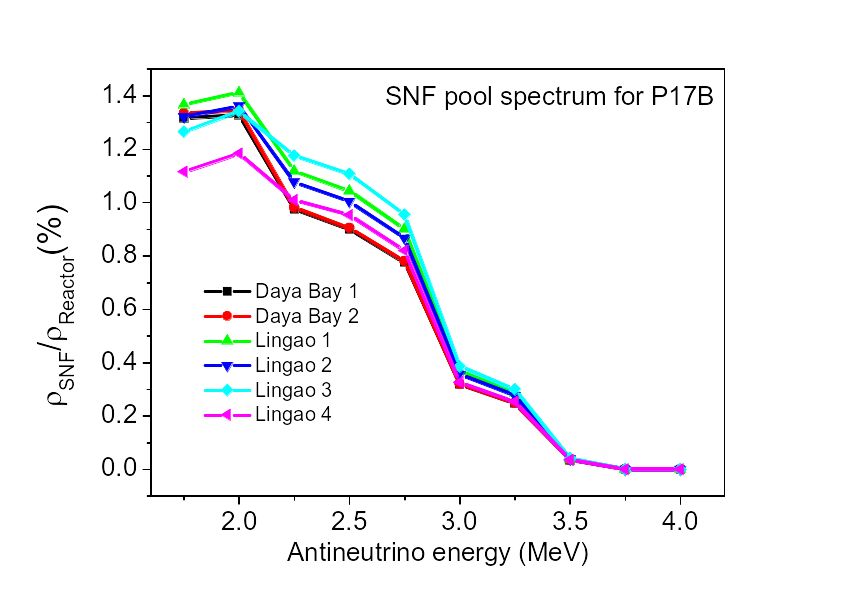
\includegraphics[width=0.72\textwidth]{Reactor/snfSpectra.png}
  \caption{The spectrum of antineutrinos from each pool of spent nuclear fuel, relative to the spectrum of antineutrinos from the corresponding core. From \cite{p17bSnf}.}
    \label{fig:reacSnfSpectra}
\end{figure}

\section{Power, burnup, and fission fractions}
\label{sec:reacpow}

In order to combine the various ingredients above into a final reactor antineutrino prediction, we must know the generated thermal power of each core, its fission fractions, and its refueling history. This information is provided by the power company in a number of forms.

Each core's average daily thermal power is provided as a fraction of the full nominal power (2895~MW). This information is crucial for calculating the fission fractions (discussed below), but the Daya Bay detectors do not always produce a full 24~hours of ``good'' data each day. As such, the collaboration periodically supplies the power company with a ``good hour'' list, from which the company produces a livetime-averaged daily power. Combined with the daily livetime, this provides a normalization for the daily predicted spectrum at each detector.

The fission fractions of a core can be expressed as a function of \emph{burnup} (\autoref{fig:reacFissionFrac}). Burnup is defined as the total energy extracted from each unit mass of fuel, typically given in units of MWd/(Metric Ton Uranium). The power company has performed simulations to determine the fission fractions versus burnup of each core\footnote{Data is provided for a full fuel cycle; for cycles that haven't yet run their course, nominal projections of thermal power are used for the ``future'' fractions.}, and this information is provided to the collaboration in intervals of $\sim$1000~MWd/MTU. The company also provides the burnup of each core at two-week intervals; using the daily generated thermal power to interpolate between the provided points, the daily burnup, and hence fission fractions, can be calculated.

% [XXX How do we deal with the fact that each core contains three batches at different burnups? See Christine's code.]

\section{Final AD spectrum}
\label{sec:adspectra}

Putting it all together, the predicted IBD spectrum at a given detector, from a single core, is
\begin{equation}
  S_{\mathrm{ibd}}(E, t) = \frac{N_p(t)}{4\pi L^2} \, \epsilon(E, t) \,
    \sigma(E) \left( \sum_i \left( \frac{W(t) \, f_i(t)}{\sum_i f_i(t) \, e_i}
        S_i(E) \, c_{\mathrm{ne},i}(E, t) \right) + S_{\mathrm{snf}}(E, t)
    \right).
\end{equation}
Here, $E$ is the \nubar energy, not the IBD prompt energy; $N_p(t)$ is the number of target protons; $L$ is the baseline; $\epsilon(E, t)$ is the detection efficiency; $\sigma(E)$ is the IBD cross section; $W(t)$ is the thermal power; $f_i(t)$ is the fission fraction of isotope $i$, $e_i$ is its energy per fission (\autoref{tab:reacEnergyPerFission}), $S_i(E)$ is its per-fission spectrum, and $c_{\mathrm{ne},i}(E, t)$ is its non-equilibrium correction; and finally, $S_\mathrm{snf}(E, t)$ is the spectrum from spent fuel. The full prediction at each detector is obtained by adding the contributions from each core.

\begin{table}[ht]
  \begin{tabular}{lcccc}
    \toprule
    & $^{235}$U & $^{238}$U & $^{239}$Pu & $^{241}$Pu \\
    \midrule
    Energy (MeV) & $201.92 \pm 0.46$ & $205.52 \pm 0.96$ & $209.99 \pm 0.60$ & $213.60 \pm 0.65$ \\
    \bottomrule
  \end{tabular}
  \caption{Energy per fission of the four main fuels in a pressurized water reactor \cite{Kopeikin_2004}.}
  \label{tab:reacEnergyPerFission}
\end{table}
% Note, according to PhysRevC.88.014605, 209.99 should be 210.99, but we've been using 209.99. In the long paper we refer to the newer calculations from PhysRevC.88.014605.

\section{Covariance matrix}
\label{sec:reacunccorr}

The uncertainties of the reactor antineutrino spectra exhibit significant correlations between energy bins, isotopes, and reactor cores. As such, it would be inappropriate to simply assign an independent error bar to each energy bin of the predicted spectra. Instead, a full covariance matrix is needed in order to account for the correlations. Such a covariance matrix was generated by taking into account the following uncertainties \cite{Lewis}:

\begin{itemize}
\item The uncertainties in the $^{235}$U, $^{239}$Pu, and $^{241}$Pu spectra resulting from the statistics of the ILL measurements and from the biases of the conversion procedure \cite{PhysRevC.84.024617}. These are uncorrelated between energy bins and isotopes, but correlated between cores.
\item The uncertainties in the $^{235}$U, $^{239}$Pu, and $^{241}$Pu spectra resulting from nuclear physics (Coulomb and weak magnetism corrections) \cite{PhysRevC.84.024617}. These are completely correlated between energy bins, isotopes, and cores.
\item The uncertainties in the $^{238}$U spectrum, primarily due to missing information in the nuclear databases \cite{PhysRevC.83.054615}. These are conservatively treated as correlated between energy bins and cores.
\item The uncertainties of the energies per fission (\autoref{tab:reacEnergyPerFission}). The errors are assumed to be Gaussian, and uncorrelated between isotopes, but correlated between cores.
\item The uncertainties in the fission fractions determined from data provided by the power company. Based on comparisons of simulations and measurements of spent fuel rods, an uncertainty of 5\% is assigned, correlated between cores.
\item The uncertainties in the generated thermal power reported by the power company. Monthly measurements of power were taken using an offline heat-balance system with an 0.48\% uncertainty. The daily power measurements for each core, in turn, were taken using an online system calibrated to the offline one, with an 0.1\% calibration error. As such, the reactor power uncertainty is assigned to be 0.1\% uncorrelated and 0.5\% correlated between cores.
\item The 30\% uncertainties in the non-equilibrium correction factors from \cite{PhysRevC.83.054615}. These are correlated between energy bins and cores, but uncorrelated between isotopes.
\item The uncertainties in the SNF spectra. An uncertainty of 100\%, correlated between spent fuel pools and energy bins, is assigned, as well as an additional 100\% uncertainty correlated between energy bins but not between pools (to account for the uncertainty in the quantity of spent fuel in each pool).
\end{itemize}

A large sample of $M$ simulated total reactor antineutrino spectra was simulated\footnote{The exact value of $M$ is unspecified in \cite{Lewis} or in the associated code, but presumably it was large enough for convergence of the covariance matrix.}, with random fluctuations applied according to the uncertainties listed above \cite{Lewis}. The covariance matrix was then calculated according to
\begin{equation}
  V_{ij} = \frac{1}{M} \sum_{n=1}^M(S^n_{i} - S^0_{i})(S^n_{j} - S^0_{j}),
\end{equation}
where the indices $i$ and $j$ run over the energy bins (each of 50~keV) and cores, the index $n$ runs over the simulated spectra, $S^n$ is the $n$th simulated spectrum, and $S^0$ is the nominal spectrum. The covariance matrix $V_{ij}$ is then used in this analysis's toy Monte Carlo in order to fluctuate the toy reactor $\nuebar$ spectra used in generating the signal systematic covariance matrix, as discussed in \autoref{sec:fitToyOutputs}.

\end{document}